%For a long time, relational database management systems (RDBMS) used to be the ?one size fits all? solution. From business data processing to analytics and data warehousing, any application could meet all of its requirements using only a SQL database. Since the early 2000's, the data 

% SQL once was the "one size for all" option
In the 1970's, the relational database management systems (RDBMS) were invented to solve the business transaction processing problem, in which data object needed to be stored and retrieved from disk efficiently for the first time. % System R citation
Between the 1970's and the 2000's, RDBMS have shown to become quite versatile and applicable to a number of number of other fields such as data warehousing, information retrieval... Such versatility made it convenient and appropriate to consider RDBMS a "one size fits all" solution, and build applications used a SQL database to handle all of its data management needs.

% SQL limitations
However, RDBMS do have their limitations. First, when the volume of data to be stored or the throughput of operation becomes too high, a system can either scale vertically (by getting a bigger machine) or horizontally (by getting more machines). A relational database doesn't scale well horizontally, and there is a limit of how big a single machine can become (bigger machine are quite expensive as well). Second, relational databases are restricted to a fixed schema which describes how the data is stored, and a change to the schema is difficult to perform, especially in an already running system. Finally, relational databases are based on the relational data and query model, and when the data and query model of an application becomes too different from the relational model, queries becomes too complex to express and too slow during execution.

% Specialized systems and their emergence.
In the early 2000's, the limitations of RBMS became more obvious as the number of applications grew exponentially. Stream processing required maintaining queries continuously despite a high insert rate, graph analysis and warehousing analytics required answering queries based on edges and columns respectively, rather than rows. Later in the mid-2000's, the volume and velocity of data for some applications became so high that horizontal scaling became a necessity and relational databases could not keep up with the performance requirements.
Likewise, the need for complex analytics over large amounts of data required the horizontal scalability and flexibility that only systems based on the Map Reduce ~\cite{Dean2008} paradigm could offer. As a result, specialized systems emerged for each of those fields and quite naturally outperformed RDBMS in their own field of specialization. Stonebreaker \& al, showed that even in the field of business transaction processing, the very problem were conceived for, RDBMS are outperformed by H-Store ~\cite{Stonebreaker2007}, a specialized system. The "one size fits all" paradigm requires RDBMS to perform decently under very different workload scenarios, making trade-offs when specialized systems did not need to make them. Figure ~\ref{fig:dblandscape} shows a recent landscape of specialized systems ~\cite{Aslett2012}.

\begin{figure}
 \centering
  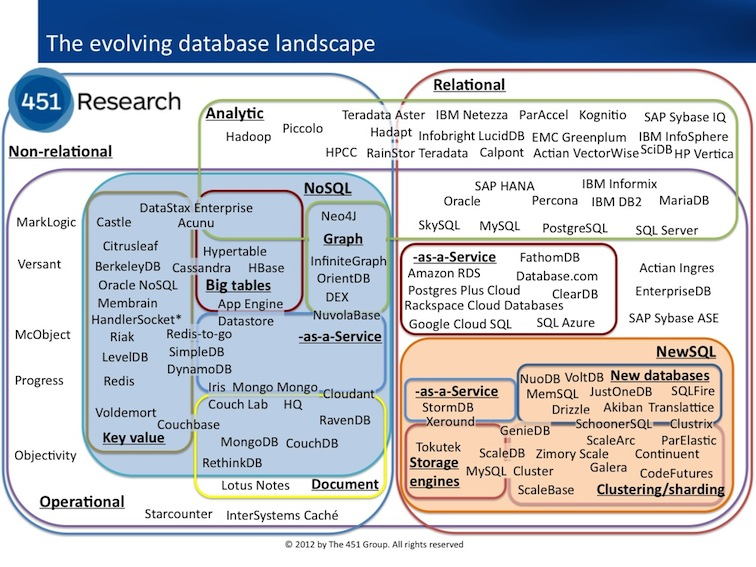
\includegraphics[width=0.8\textwidth]{images/DBlandscape.jpg}
  \caption{Landscape of database systems available as of late 2012, many of which are very recent.}
  \label{fig:dblandscape}
\end{figure}


%TODO : check that it is not a problem to reuse part of an article if we explicitly cite it. 
% Polyglot Persistence
The downside of having specialization is that naturally applications arise where an application's requirements aren't met by any single specialized system. Two approaches exist to solve this problem. The first option is to take an existing specialized system capable of doing $X$, and understand how to extend it to make it able to $Y$. Lim \& al ~\cite{Lim2013} provide three examples of such systems : i) \emph{MapReduce Online}, which adds pipelining and stream processing to the batch-oriented Map Reduce framework ~\cite{Condie2010}; ii) \emph{Online Aggregation for Map Reduce} which adds approximate answering capabilities to MapReduce ~\cite{Pansare2011}; HadoopDB, which enhances MapReduce's performance for SQL query processing while retaining MapReduce's fault-tolerance and fine-grained adaptivity ~\cite{Abouzeid2009}. This approach seems to consider going back to "one size fits all" systems, which begs the question how such systems will avoid the problems the RDBMS are confronted to.

In this paper, we take a different approach called "Polyglot Persistence" (PP) ~\cite{Fowler2012},  in which multiple specialized systems are used in coordination in order to meet all the requirements. Enabling such a coordination creates a number of challenges since specialized systems have been built to run independently and now have to be integrated together despite differing on a number of logical and architectural dimensions. We present those challenges here :

%Challenges
\begin{enumerate}
% TODO : warning, potential copyright infringement, reusing sentence from other paper.
\item{\emph{Choosing which systems to integrate given a set of requirements} : as seen on Figure ~\ref{fig:dblandscape}, the number of options is already large and growing larger every day. For a given application requirement, it isn't always clear which option is the best. Should the application developer use a SQL or NoSQL system? Within NoSQL, should she use a key-value store, a document database or column family system? How much more performance increase will a two-system solution provide over a one-system solution? How much more of a complexity overhead will a two system solution incur over a one system solution? As Lim \& al ~\cite{Lim2013}  point out, benchmarking storage options is not easy, in particular when application requirements are not quite set in stone yet.}
\item{How do we integrate multiple specialized system into a PP system?}
\item{How do we optimize queries in a PP system?}
\item{How do we provision resources for each specialized system?}
\item{How do we store data in a PP system?}
\item{How do we update the PP system?}
\item{How do we keep the PP system available and consistent?}
\item{How do we deal with changes in the requirements of the application using the PP system?}
\end{enumerate}
